\problemname{Rullband}
Det svenska laget till Internationella Programmeringsolympiaden har just landat i Singapore för att
tävla i \href{https://ioi2020.sg/}{IOI 2020}.
På vägen till bagageupphämtningen ska de genom en lång korridor med massa rullband.
Korridoren är $M$ meter lång, och laget står just nu i början av den och funderar på
hur snabbt de kan ta sig till bagageupphämtningen.
Det finns $N$ \href{https://sv.wikipedia.org/wiki/Rullande_trottoar}{rullband} i korridoren.
Varje rullband börjar på ett visst avstånd från början av korridoren,
slutar på ett visst avstånd från början av korridoren och tar en viss tid att åka längs.
Alla rullband går i korridorens riktning, och man kan endast kliva på ett rullband i början av det och endast kliva av vid slutet av det.
När laget inte går på något rullband tar det $g$ sekunder att gå en meter.
Korridoren och rullbanden är så pass smala att endast tiden det tar att gå
parallellt med korridoren spelar roll. 
Alltså, ifall ett rullband slutar samma avstånd från början
som ett annat rullband början så tar det ingen tid att gå mellan
rullbanden. Vad är den snabbate tiden laget kan ta sig genom hela korridoren på?

Notera att det kan vara gynnsamt att ibland gå lite bakåt genom korridoren för att komma på
ett rullband som tar en långt fram. Det finns dock inga rullband som går bakåt genom
korridoren.

\section*{Indata}
Den första raden innehåller tre heltal $N$, $M$, $g$ ($1 \le N \le 2\times10^5$, $2 \le M \le 2\times10^5$, $1 \le g \le 100$):
antal rullband, längden på korridoren i meter, och lagets gånghastighet i sekunder per meter.
De följande $N$ raderna beskriver rullbanden och innehåller 3 heltal vardera: $s_i, e_i$ och $t_i$
($1\leq s_i,e_i\leq M,1\leq t_i\leq100$).
$s_i$ är antal meter från början av korridoren till rullbandets början, $e_i$ är antal meter
från början av korridoren till rullbandets slut och $t_i$ är hur lång tid det tar att åka längs rullbandet.

\section*{Utdata}
Skriv ut en rad med ett heltal: antal sekunder det tar för laget att komma genom korridoren.

\section*{Poängsättning}
Din lösning kommer att testas på en mängd testfallsgrupper.
För att få poäng för en grupp så måste du klara alla testfall i gruppen.

\noindent
\begin{tabular}{| l | l | l |}
\hline
Grupp & Poängvärde & Gränser \\ \hline
1     & 8          &  $N,M \le 10$ och man behöver aldrig gå bakåt\\ \hline
2     & 13         &  $N,M \le 1000$ och man behöver aldrig gå bakåt\\ \hline
3     & 40         &  $N,M \le 2\times10^5$ och man behöver aldrig gå bakåt\\ \hline
4     & 15         &  $N,M \le 1000$. \\ \hline
5     & 24         &  Inga ytterligare begränsningar. \\ \hline
\end{tabular}

\section*{Förklaring av exempelfall}

\begin{figure}[h]
	\centering
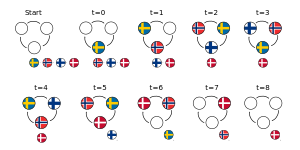
\includegraphics[width=0.7\textwidth]{sample1}
\caption{Exempelfall 1}
\end{figure}
I exempelfall 1 tar det 2 sekunder att gå en meter när laget inte går på något rullband.
Det snabbaste sättet att ta sig till slutet är att gå till rullbandet som
tar 5 sekunder, åka på det, gå till det som tar 2 sekunder och sen åka på det.
Totala tiden detta tar är $4+5+2+2=13$ sekunder.



\begin{figure}[h]
	\centering

\includegraphics[width=0.7\textwidth]{sample2}
\caption{Exempelfall 2}
\end{figure}
I exempelfall 2 tar det istället 5 sekunder att gå en meter när laget inte går på något rullband.
Det snabbaste sättet att ta sig till slutet är att gå till rullbandet som
tar 8 sekunder, åka på det, gå tillbaka en meter och åka på
rullbandet som tar 2 sekunder, och sen gå sista metern.
Totala tiden detta tar är $5+8+5+2+5=25$ sekunder.
